
%(BEGIN_QUESTION)
% Copyright 2011, Tony R. Kuphaldt, released under the Creative Commons Attribution License (v 1.0)
% This means you may do almost anything with this work of mine, so long as you give me proper credit

This single-loop flow control system has a problem: the flow rate indicated on the controller's faceplate shows it to be precisely at setpoint (250 SCFM), yet the Annubar flow gauge does not agree.  The two indications used to agree with one another just fine, until some time recently.

$$\includegraphics[width=15.5cm]{i03480x01.eps}$$

Determine the diagnostic value of each of the following tests.  Assume only one fault in the system, including any single component or any single wire/cable/tube connecting components together.  If a proposed test could provide new information to help you identify the location and/or nature of the one fault, mark ``yes.''  Otherwise, if a proposed test would not reveal anything relevant to identifying the fault (already discernible from the measurements and symptoms given so far), mark ``no.''

% No blank lines allowed between lines of an \halign structure!
% I use comments (%) instead, so that TeX doesn't choke.

$$\vbox{\offinterlineskip
\halign{\strut
\vrule \quad\hfil # \ \hfil & 
\vrule \quad\hfil # \ \hfil & 
\vrule \quad\hfil # \ \hfil \vrule \cr
\noalign{\hrule}
%
% First row
{\bf Diagnostic test} & {\bf Yes} & {\bf No} \cr
%
\noalign{\hrule}
%
% Another row
Measure AC line voltage &  &  \cr
%
\noalign{\hrule}
%
% Another row
Measure DC power supply output voltage &  &  \cr
%
\noalign{\hrule}
%
% Another row
Inspect PID tuning parameters in controller &  &  \cr
%
\noalign{\hrule}
%
% Another row
Check pressure transmitter calibration &  &  \cr
%
\noalign{\hrule}
%
% Another row
Measure transmitter current signal &  &  \cr
%
\noalign{\hrule}
%
% Another row
Put controller into manual mode and move valve &  &  \cr
%
\noalign{\hrule}
%
% Another row
Measure DC voltage between TB1-3 and TB1-4 &  &  \cr
%
\noalign{\hrule}
%
% Another row
Measure DC voltage between TB1-7 and TB1-8 &  &  \cr
%
\noalign{\hrule}
} % End of \halign 
}$$ % End of \vbox

\vfil 

\underbar{file i03480}
\eject
%(END_QUESTION)





%(BEGIN_ANSWER)

This is a graded question -- no answers or hints given!

%(END_ANSWER)





%(BEGIN_NOTES)

Since the problem we face here is a discrepancy between the Annubar gauge's indication of flow and the transmitter's indication of flow, we must limit our diagnostic tests to those which will specifically probe possible faults in either the Annubar gauge or in the transmitter/sensing portion of the circuit.

\vskip 10pt

Clearly, a problem could exist in the Annubar gauge.  Alternatively, a problem could exist in the transmitter, the 4-20 mA measurement signal circuit, or the controller itself.  When diagnosing problems in a measurement system such as this where multiple components must work in serial fashion to convey information from one place to another, it is prudent to as yourself whether each one of those components is receiving/transmitting properly.  For example, while it is possible that the transmitter itself has a calibration error and therefore outputs the wrong signal to the controller, it is just as possible that the transmitter is indeed sending the correct signal, but that the controller is not interpreting that signal correctly, and instead is displaying something different.

\vskip 10pt

This is why checking the transmitter's calibration or measuring its output signal are both good tests.  Similarly, measuring voltage across the resistor would also reveal the signal going into the controller, which in turn would tell you whether the problem was in the controller or in the signal being sent to it.

% No blank lines allowed between lines of an \halign structure!
% I use comments (%) instead, so that TeX doesn't choke.

$$\vbox{\offinterlineskip
\halign{\strut
\vrule \quad\hfil # \ \hfil & 
\vrule \quad\hfil # \ \hfil & 
\vrule \quad\hfil # \ \hfil \vrule \cr
\noalign{\hrule}
%
% First row
{\bf Diagnostic test} & {\bf Yes} & {\bf No} \cr
%
\noalign{\hrule}
%
% Another row
Measure AC line voltage &  & $\surd$ \cr
%
\noalign{\hrule}
%
% Another row
Measure DC power supply output voltage &  & $\surd$ \cr
%
\noalign{\hrule}
%
% Another row
Inspect PID tuning parameters in controller &  & $\surd$ \cr
%
\noalign{\hrule}
%
% Another row
Check pressure transmitter calibration & $\surd$ &  \cr
%
\noalign{\hrule}
%
% Another row
Measure transmitter current signal & $\surd$ &  \cr
%
\noalign{\hrule}
%
% Another row
Put controller into manual mode and move valve & $\surd$ &  \cr
%
\noalign{\hrule}
%
% Another row
Measure DC voltage between TB1-3 and TB1-4 & $\surd$ &  \cr
%
\noalign{\hrule}
%
% Another row
Measure DC voltage between TB1-7 and TB1-8 &  & $\surd$ \cr
%
\noalign{\hrule}
} % End of \halign 
}$$ % End of \vbox

Moving the valve in manual mode will be a worthwhile test {\it only} if you also check the gauge's and controller's indications of pressure with the valve in a different position.  The purpose of this test is to see whether or not the gauge or the transmitter are ``stuck'' at one reading.  Both indications should change with a change in valve position.  If one of them does not change, you've found the ``stuck'' instrument.


\filbreak

$$\includegraphics[width=15.5cm]{i03480x02.eps}$$

\filbreak \vskip 20pt \vbox{\hrule \hbox{\strut \vrule{} {\bf Virtual Troubleshooting} \vrule} \hrule}

\noindent
{\bf Predicting the effect of a given fault:} present each of the following faults to the students, one at a time, having them comment on all the effects each fault would produce.

\begin{itemize}
\item{} Valve $V_3$ left open
\item{} 250 $\Omega$ resistor failed open
\item{} Loss of instrument air supply to I/P converter
\item{} Power supply failed with zero DC output voltage
\item{} Bypass valve left open
\item{} Open wire between FIC-91 and FY-91
\end{itemize}


\vskip 10pt


\noindent
{\bf Identifying possible/impossible faults:} present symptoms to the students and then have them determine whether or not a series of suggested faults could account for all the symptoms, explaining {\it why} or {\it why not} for each proposed fault:

\begin{itemize}
\item{} Symptom: {\it }
\item{}  -- {\bf Yes/No}
\item{}  -- {\bf Yes/No}
\item{}  -- {\bf Yes/No}
\end{itemize}


\vskip 10pt


\noindent
{\bf Determining the utility of given diagnostic tests:} present symptoms to the students and then propose the following diagnostic tests one by one.  Students rate the value of each test, determining whether or not it would give useful information (i.e. tell us something we don't already know).  Students determine what different results for each test would indicate about the fault, if anything:

\begin{itemize}
\item{} Symptom: {\it }
\item{}  -- {\bf Yes/No}
\item{}  -- {\bf Yes/No}
\end{itemize}


\vskip 10pt


\noindent
{\bf Diagnosing a fault based on given symptoms:} imagine the ??? fails ??? in this system (don't reveal the fault to students!).  Present the operator's observation(s) to the students, have them consider possible faults and diagnostic strategies, and then tell them the results of tests they propose based on the following symptoms, until they have properly identified the nature and location of the fault:

\begin{itemize}
\item{} Operator observation: {\it }
\item{} 
\item{} 
\end{itemize}
%INDEX% Troubleshooting review: electric circuit diagnostic test usefulness

%(END_NOTES)


